\chapter*{Example Mapping}

\ifnotes
    
    This is possibly the most important part of the day. Spend time making sure it works.
    
    As an alternative, for more energy and less time, you can facilitate a discussion that draws on the ATM examples exercise to derive the core concepts of example mapping from first principles. Then let the delegates know that the full description of Example Mapping is available online.
    
    Learning outcomes:
    
    \begin{itemize}
        \item Describe the practical process of example mapping like card colours and map structure
        \item Explain the purpose of Example Mapping
    \end{itemize}
\fi 

\ifcontent
    Example Mapping is a discovery technique discovered by Matt Wynne. It's documented in full online \footnote{https://cucumber.io/blog/2015/12/08/example-mapping-introduction}. Today we're going to learn the key points of example mapping. 
    
    \begin{framed}
       Before you pull a user story into development, it’s crucial to have a conversation to clarify and confirm the acceptance criteria.

        Some people do this during their backlog refinement or planning poker sessions. Other teams have a specific three amigos meeting, specification workshop or discovery workshop. Whatever you call this conversation, many teams find it hard; it’s unstructured, it takes too long and gets boring. The result is they don’t do it regularly or consistently, or maybe they just give up on it entirely.
        
        Example Mapping uses concrete examples to help us explore the problem domain, and they make a great basis for our acceptance tests. But as we discuss these examples, there are other things coming out in the conversation that deserve to be captured too:
        
        \begin{itemize}
            \item rules that summarise a bunch of examples, or express other agreed constraints about the scope of the story.
            \item questions about scenarios where nobody in the conversations knows what the right outcome is. Or assumptions we're making in order to progress.
            \item new user stories we discovered or sliced and deferred out of scope.
        \end{itemize} 
       
       \begin{flushright}
            \textit{Matt Wynne, Introducing Example Mapping}
        \end{flushright}
    \end{framed}
    
    
    Here's a picture of an example map midway through construction:
    
    \begin{center}
        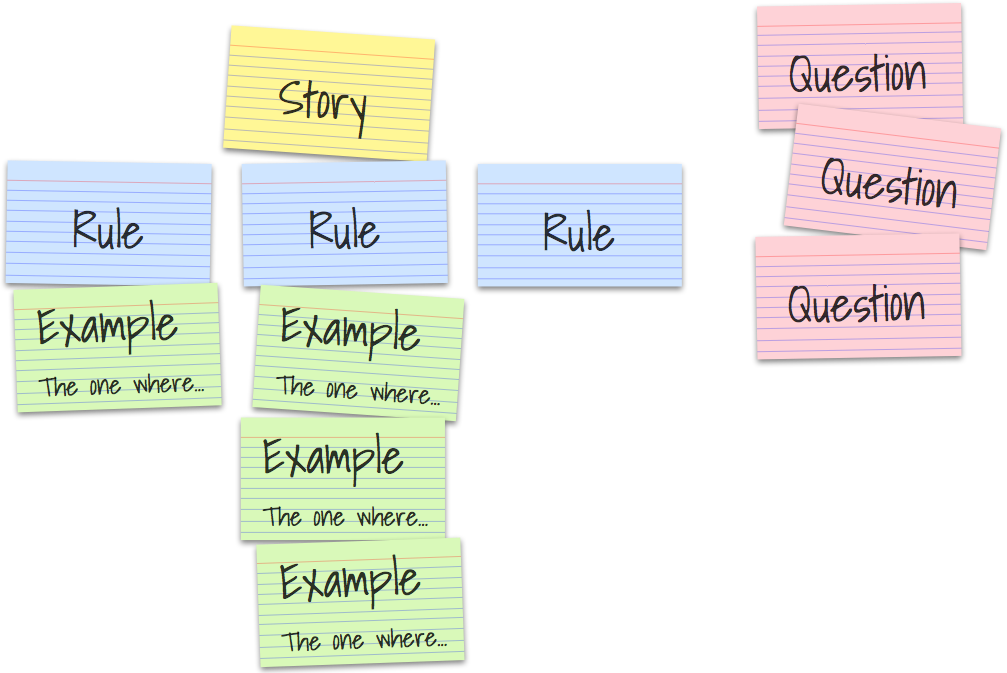
\includegraphics[width= 0.6\textwidth]{bdd-fundamentals/images/example-map.png} 
    \end{center}

\fi 


\chapter*{Try it out}

\ifnotes

    \section*{Learning outcomes}
    
    \begin{itemize}
        \item Experience the practical application of Example Mapping

    \end{itemize}
    
    
    \section*{Setup}

    This needs strong facilitation. It's hard and neither the product owner nor the team have any domain knowledge. Emphasise:
    
    \begin{itemize}
        \item the PO is "empowered" and can make any decision they like
        \item there are some rules in the product concept
        \item the whole team should come up with \& write examples
        \item the initial use case
        \item examples can be written in any format (NOT G/W/T)
    \end{itemize}   
    
    
    \section*{Review}
    
    Ask room - "what's the purpose of Example Mapping?" Suggestions include:
    
    \begin{itemize}
        \item Discover what you don't know
        \item Discover new rules
        \item Refine known rules
        \item Get on the same page
        \item Establish a shared vocabulary
        \item Design tests
        \item Break down user stories
        \item Build empathy, avoid finger pointing - everyone gave their best shot
        \item Avoid starting to implement stories that aren't ready (thumb vote, Definition of Ready)
    \end{itemize}

    Ask room - "how can you split stories?"
    
    \begin{itemize}
        \item each rule can become a new (small) story to put on backlog 
        \item in the handout, at the back, is the How To Split A User Story graphic. Let them know it's freely available online. Looking at an example map is only one way to split a story.
    \end{itemize}

    
\fi 


\ifcontent

    Now we're going to try it out for ourselves.
    
    Break into groups of 3-4 and nominate a product owner, who will make decisions about the direction the product will take. Other members of your group can take the roles of developer or tester for the purpose of the exercise.
    
    Everyone should now read the product concept document from Appendix 1.
    
    Your goal is to run an example mapping session to help discover what the development team should work on. 
    
    Start the conversation by discussing the rules described in the product concept document. Write the rules on blue index cards. Capture \emph{concrete} examples that illustrate the rules on green index cards in below them.
    
    What user story describes the value that implementing these rules would deliver? Write that on a yellow index card.
    
    Did you think of any examples that aren't covered by the rules already described? Write any rules you discover on blue index cards. 
    
\fi